\documentclass[preview]{standalone}

\usepackage{amsmath}
\usepackage{amssymb}
\usepackage{stellar}
\usepackage{bettelini}
\usepackage{wrapfig}

\hypersetup{
    colorlinks=true,
    linkcolor=black,
    urlcolor=blue,
    pdftitle={Biologia},
    pdfpagemode=FullScreen,
}

\begin{document}

\title{Biologia}
\id{biologia-respirazione-cellulare}
\genpage

\section{Respirazione cellulare}

\begin{snippet}{respirazione-cellulare-expl}
    Nella respirazione cellulare, il glucosio è demolito fino alle semplici molecole CO\({}_2\) e H\({}_2\)O,
    mentre viene consumato O\({}_2\). L'energia che si libera viene immagazzinata nelle molecole di
    ATP che sono utilizzate poi dalla cellula per svolgere i diversi processi metabolici. Come in
    tutte le trasformazioni energetiche, anche in questo caso parte dell'energia è dissipata come
    calore. La respirazione cellulare include una serie di reazioni in cui si distinguono tre tappe
    principali: la \textit{glicolisi}, \textit{il ciclo di Krebs} e la \textit{fosforilazione ossidativa}.
    L'ultima tappa comprende a sua volta due processi:
    la \textit{catena di trasporto degli elettroni} e la \textit{chemiosmosi}. Nelle cellule
    eucariote la glicolisi si svolge nel citoplasma, il ciclo di Krebs nella matrice mitocondriale e
    la fosforilazione ossidativa nella membrana interna dei mitocondri; nei procarioti le prime
    fasi avvengono nel citoplasma e la catena di trasporto degli elettroni è incorporata nella
    membrana plasmatica
\end{snippet}

\includesnpt[width=70\%|src=/snippet/static/respirazione-cellulare.png]{centered-img}

\begin{snippetdefinition}{mitocondrio-definition}{Mitocondrio}
    Il \textit{mitocondrio} è un organello nella cellula dove avviene parte della respirazione cellulare.
\end{snippetdefinition}

\plain{Il mitocondrio è composto da due membrane, dividendosi in una parte interna ed esterna.}

\begin{snippetdefinition}{creatina-definition}{Creatina}
    La \textit{creatina} è una molecola che possiede un fosfato, il suo scopo è quello di aumentare la produzione di ADP.
\end{snippetdefinition}

\subsection{Glicolisi}

\begin{snippetdefinition}{glicolisi-definition}{Glicolisi}
    La \textit{glicolisi} è una serie di reazioni chimiche che spaccano il glucosio in 2 \textit{piruvati} (\(C_3H_6O_3\)).
\end{snippetdefinition}

\begin{snippet}{glicolisi-expl}
    La glicolisi scinde la molecola di glucosio (con sei atomi di carbonio) in due molecole di
    piruvato, con tre atomi di carbonio (C\({}_3\)H\({}_6\)O\({}_3\)). È un processo anaerobico, cioè che non
    richiede ossigeno, e comprende una serie di reazioni durante le quali la cellula produce due
    molecole di NADH e due molecole di ATP, ricche di energia. I lieviti e alcuni batteri possono
    soddisfare il proprio fabbisogno di energia esclusivamente grazie alla glicolisi. La maggior
    parte degli organismi, tuttavia, richiede molta più energia, ottenuta dai passaggi successivi
    della respirazione cellulare.
\end{snippet}

\subsection{Il ciclo di Krebs}

\begin{snippet}{ciclo-di-krebs-expl}
    Il piruvato, il prodotto finale della glicolisi, subisce alcune modificazioni chimiche prima di
    passare dal citoplasma ai mitocondri per prendere parte al ciclo di Krebs. In queste
    trasformazioni, per ogni molecola di glucosio che prende parte alla glicolisi vengono
    sintetizzate due molecole di acetilcoenzima A (o acetil-CoA) e altre due molecole di NADH.
    Soltanto il gruppo acetile a due atomi di carbonio della molecola di acetil-CoA partecipa
    effettivamente al ciclo, mentre il coenzima A si stacca per essere riciclato. Poiché nel ciclo
    di Krebs entrano due molecole di acetil-CoA per ogni molecola iniziale di glucosio, la
    produzione complessiva è di 2 ATP, 6 NADH e 2 FADH\({}_2\) per ciascuna molecola di glucosio.
    Dopo la glicolisi e il ciclo di Krebs, la cellula ha dunque a disposizione un totale di 4 ATP, 10
    NADH e 2 FADH\({}_2\). L'ATP prodotto è poco, ma la principale funzione delle prime due tappe
    della respirazione cellulare è alimentare la fosforilazione ossidativa tramite le molecole di
    NADH e FADH\({}_2\).
\end{snippet}

\includesnpt[width=45\%|src=/snippet/static/ciclo-di-krebs.png]{centered-img}

\subsection{La fosforilazione ossidativa}

\begin{snippet}{fosforilazione-ossidativa-expl}
    La fosforilazione ossidativa, che avviene sulla membrana interna dei mitocondri, comprende
    la catena di trasporto degli elettroni e la chemiosmosi. Nella catena di trasporto degli
    elettroni il NADH e il FADH\({}_2\) cedono elettroni a un complesso di molecole che li trasportano
    fino all'ossigeno. Ciascun atomo di ossigeno accetta due elettroni dalla catena di trasporto
    e due ioni H\({}^+\) dalla soluzione circostante per formare H\({}_2\)O, uno dei prodotti finali della
    respirazione cellulare. La chemiosmosi sfrutta l'energia liberata dai trasferimenti di elettroni
    lungo la catena di trasporto per generare ATP. Tre complessi proteici utilizzano l'energia
    liberata dalla catena di trasporto per trasportare attivamente ioni H\({}^+\) contro gradiente,
    determinando l'accumulo di energia potenziale. A questo punto l'enzima ATP sintetasi, che
    forma uno speciale complesso nella membrana interna del mitocondrio, utilizza l'energia
    potenziale per generare ATP, facendo passare gli ioni idrogeno attraverso un proprio canale.
\end{snippet}

\includesnpt[width=70\%|src=/snippet/static/fosforilazione-ossidativa.png]{centered-img}

\section{Fermantazione}

\begin{snippetdefinition}{fermentazione-definition}{Fermentazione}
    La \textit{fermentazione} è una via metabolica che permette agli esseri viventi di ricavare energia da particolari molecole organiche (carboidrati o raramente amminoacidi) in assenza di ossigeno.
\end{snippetdefinition}

\subsection{Fermantazione alcolica}

\begin{snippet}{fermentazione-alcolica-expl}
    \setlength{\intextsep}{0pt}%
    \begin{wrapfigure}{r}{6cm}
        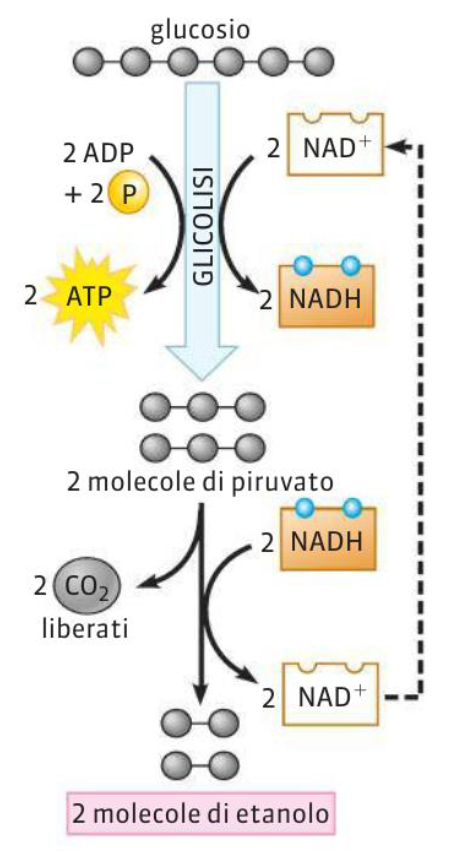
\includegraphics[width=5cm]{./resources/fermentazione-alcolica.png}
    \end{wrapfigure}
    La fermantazione alcolica viene dai lieviti e da alcuni batteri.
    
    Il piruvato viene trasformato in etanolo, in un processo che rigenera NAD\({}^+\) e produce CO\({}_2\).
    Dopo aver prodotto l'energia, è necessario sbarazzarsi del piruvato protonato (acido piruvio),
    viene quindi spaccato e scaricato nell'aria come Etanolo e CO\({}_2\).
    % CO2 e Etanolo con REDOX scaricano NADH
    \wrapfill
\end{snippet}

\subsection{Fermantazione lattica}

\begin{snippet}{fermentazione-lattica-expl}
    \setlength{\intextsep}{0pt}%
    \begin{wrapfigure}{r}{6cm}
        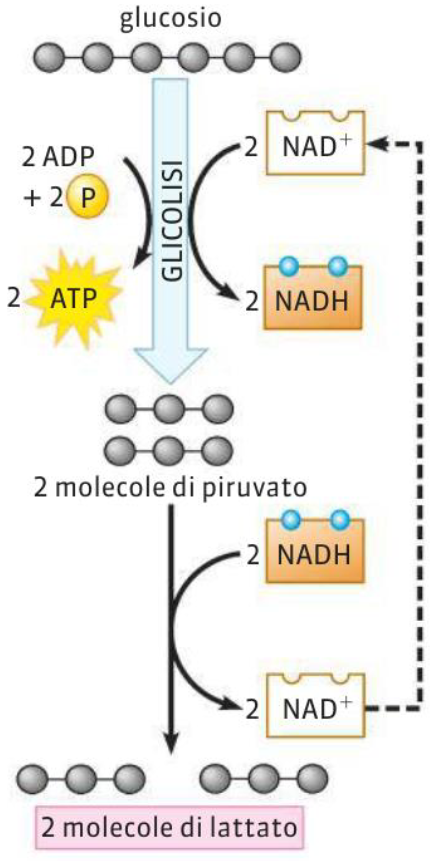
\includegraphics[width=5cm]{./resources/fermentazione-lattica.png}
    \end{wrapfigure}

    La fermentazione lattica viene svolta da alcuni organismi come batteri.
    Gli umani la svolgono dopo uno sforzo muscolare.
    Il piruvato viene convertito in acido lattico (scarto), che viene poi smaltito dal fegato con ATP.
    In questo processo si rigenera il NAD\({}^+\), la molecola a partire dalla quale
    viene prodotto il NADH durante la glicolisi.
    \wrapfill
\end{snippet}

\end{document}